% =========================================================================
% AAT — Figure: The Orient Cascade
% Companion to: #der-orient-cascade (Part II Ch.5)
%
% Build:  pdflatex orient-cascade.tex
%
% Five-step resolution order forced by information dependency. The 2x2
% diagnostic at step 3 routes the agent to step 4 (revise Sigma_t) or
% step 5 (escalate before revising O_t) or terminates at success /
% capacity-limit. Re-entry to step 1 is shown for revised M_t.
% =========================================================================
\documentclass[border=10pt]{standalone}
\usepackage{tikz}
\usepackage{amsmath,amssymb}
\usetikzlibrary{arrows.meta,positioning,calc,fit,backgrounds,shapes.geometric,shapes.symbols}

\begin{document}
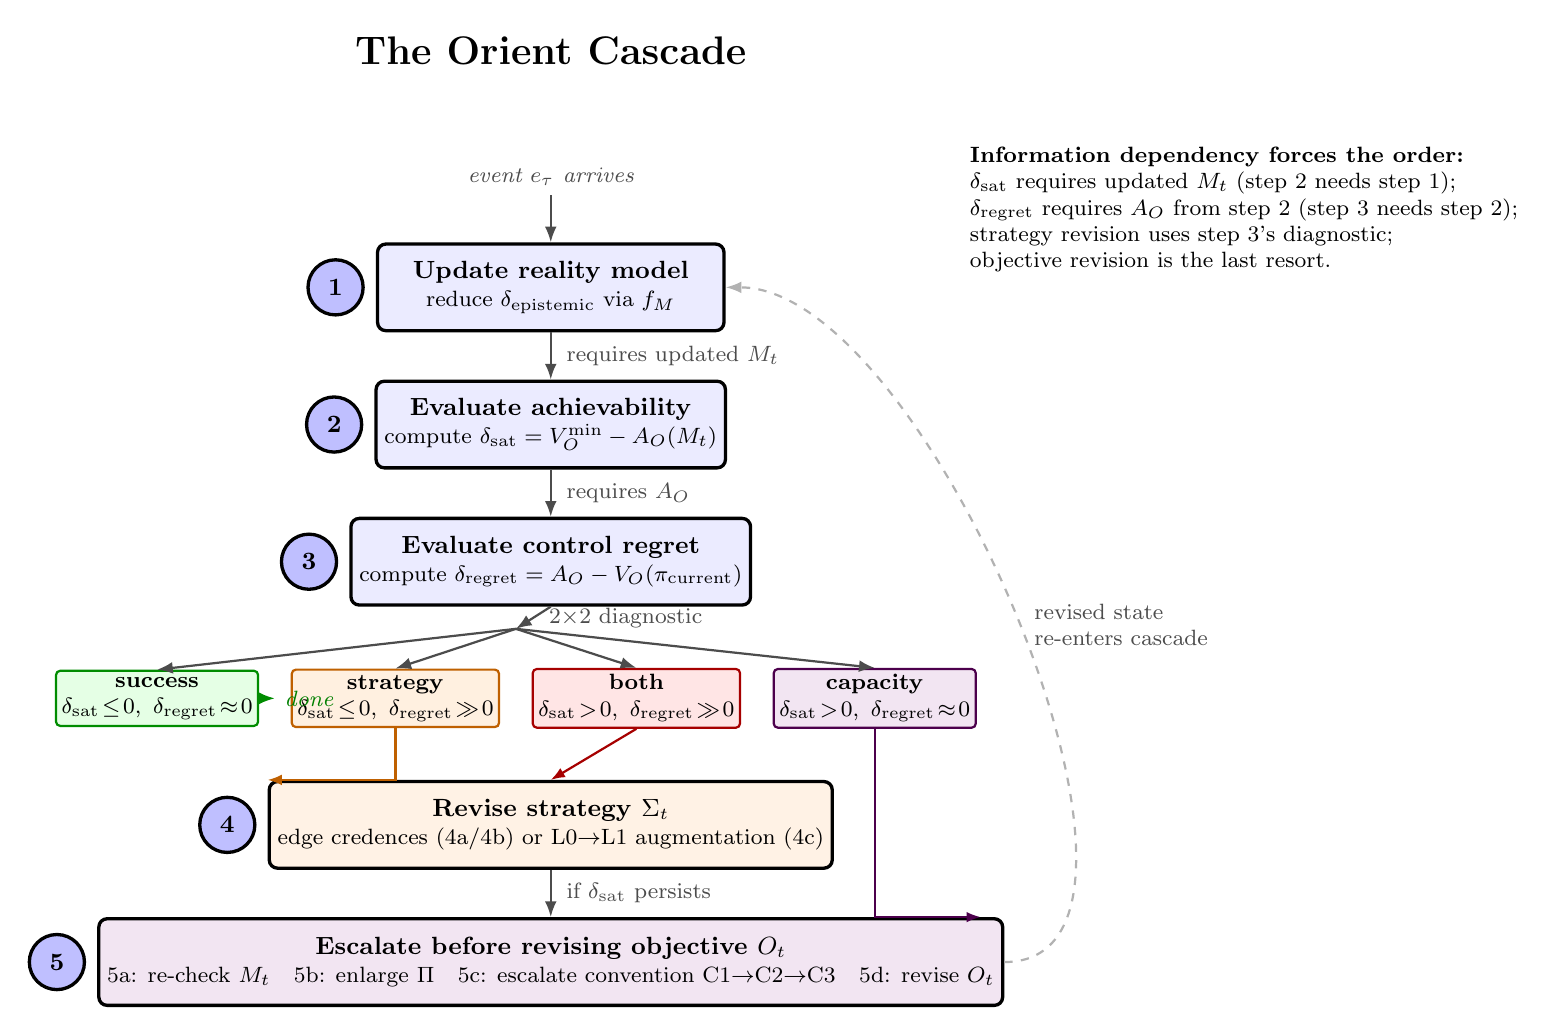
\begin{tikzpicture}[
    font=\small,
    >=Latex,
    node distance=6mm and 12mm,
    stepbox/.style       = {draw, very thick, rounded corners=3pt, fill=blue!8,
                          minimum width=4.4cm, minimum height=11mm, align=center,
                          inner sep=3pt, font=\small},
    stepnum/.style    = {circle, draw, very thick, fill=blue!25, minimum size=7mm,
                          inner sep=0pt, font=\small\bfseries},
    outcome/.style    = {draw, rounded corners=1.5pt, thick, minimum width=2.3cm,
                          minimum height=7mm, align=center, font=\footnotesize,
                          inner sep=2pt},
    succ/.style       = {outcome, fill=green!10, draw=green!55!black},
    stratp/.style     = {outcome, fill=orange!12, draw=orange!75!black},
    bothp/.style      = {outcome, fill=red!10, draw=red!65!black},
    caplim/.style     = {outcome, fill=violet!10, draw=violet!60!black},
    flow/.style       = {-{Latex[length=2mm]}, thick, black!70},
    reflow/.style     = {-{Latex[length=2mm]}, thick, gray!60, dashed},
    side/.style       = {font=\footnotesize, gray!60!black},
    branchedge/.style = {-{Latex[length=1.8mm]}, thick}
  ]

% =========================================================
% Trigger: event arrives
% =========================================================
\node[font=\footnotesize\itshape, gray!60!black] (trigger) {event $e_\tau$ arrives};

% =========================================================
% Step 1 — Update M_t
% =========================================================
\node[stepbox, below=of trigger] (s1)
  {\textbf{Update reality model} \\[-1pt]
   {\footnotesize reduce $\delta_{\text{epistemic}}$ via $f_M$}};
\node[stepnum, left=4pt of s1.west] (n1) {1};

% =========================================================
% Step 2 — Evaluate sat-gap
% =========================================================
\node[stepbox, below=of s1] (s2)
  {\textbf{Evaluate achievability} \\[-1pt]
   {\footnotesize compute $\delta_{\text{sat}} = V_{O}^{\min} - A_O(M_t)$}};
\node[stepnum, left=4pt of s2.west] (n2) {2};

% =========================================================
% Step 3 — Evaluate regret + 2x2 outcomes
% =========================================================
\node[stepbox, below=of s2] (s3)
  {\textbf{Evaluate control regret} \\[-1pt]
   {\footnotesize compute $\delta_{\text{regret}} = A_O - V_O(\pi_{\text{current}})$}};
\node[stepnum, left=4pt of s3.west] (n3) {3};

% Four outcomes of the 2x2 diagnostic (placed under step 3, side by side)
\node[succ,   below=8mm of s3.south, xshift=-5.0cm] (oA)
  {\textbf{success} \\ $\delta_{\text{sat}}\!\leq\!0,\ \delta_{\text{regret}}\!\approx\!0$};
\node[stratp, right=4mm of oA] (oB)
  {\textbf{strategy} \\ $\delta_{\text{sat}}\!\leq\!0,\ \delta_{\text{regret}}\!\gg\!0$};
\node[bothp,  right=4mm of oB] (oC)
  {\textbf{both} \\ $\delta_{\text{sat}}\!>\!0,\ \delta_{\text{regret}}\!\gg\!0$};
\node[caplim, right=4mm of oC] (oD)
  {\textbf{capacity} \\ $\delta_{\text{sat}}\!>\!0,\ \delta_{\text{regret}}\!\approx\!0$};

% =========================================================
% Step 4 — Revise Sigma_t
% =========================================================
\node[stepbox, below=22mm of s3, fill=orange!10] (s4)
  {\textbf{Revise strategy $\Sigma_t$} \\[-1pt]
   {\footnotesize edge credences (4a/4b) or L0$\rightarrow$L1 augmentation (4c)}};
\node[stepnum, left=4pt of s4.west] (n4) {4};

% =========================================================
% Step 5 — Escalate before revising O_t
% =========================================================
\node[stepbox, below=of s4, fill=violet!10, minimum width=8.0cm] (s5)
  {\textbf{Escalate before revising objective $O_t$} \\[-1pt]
   {\footnotesize 5a: re-check $M_t$\ \ \ 5b: enlarge $\Pi$\ \ \ 5c: escalate convention C1$\rightarrow$C2$\rightarrow$C3\ \ \ 5d: revise $O_t$}};
\node[stepnum, left=4pt of s5.west] (n5) {5};

% =========================================================
% Main flow arrows
% =========================================================
\draw[flow] (trigger) -- (s1);
\draw[flow] (s1) -- (s2)  node[side, midway, right=2pt]{requires updated $M_t$};
\draw[flow] (s2) -- (s3)  node[side, midway, right=2pt]{requires $A_O$};

% Step 3 -> the 4 outcomes (single arrow into the row)
\draw[flow] (s3.south) -- ($(oB.north)!0.5!(oC.north) + (0,5mm)$)
   node[side, midway, right=2pt]{2$\times$2 diagnostic};
\draw[flow] ($(oB.north)!0.5!(oC.north) + (0,5mm)$) -- (oA.north);
\draw[flow] ($(oB.north)!0.5!(oC.north) + (0,5mm)$) -- (oB.north);
\draw[flow] ($(oB.north)!0.5!(oC.north) + (0,5mm)$) -- (oC.north);
\draw[flow] ($(oB.north)!0.5!(oC.north) + (0,5mm)$) -- (oD.north);

% Routing from outcomes
% success -> done (terminate)
\node[font=\footnotesize\itshape, green!50!black, right=2mm of oA] (done) {done};
\draw[flow, green!55!black] (oA.east) -- (done);

% strategy -> step 4
\draw[branchedge, orange!75!black] (oB.south) |- (s4.north west);
% both -> step 4 (then step 5)
\draw[branchedge, red!65!black] (oC.south) -- (s4.north);
% capacity -> step 5 (skips step 4)
\draw[branchedge, violet!60!black] (oD.south) |- ($(s5.north east) + (-3mm, 0)$);

% step 4 -> step 5 (if "both")
\draw[flow] (s4) -- (s5)  node[side, midway, right=2pt]{if $\delta_{\text{sat}}$ persists};

% =========================================================
% Re-entry arrow (revised state -> back to step 1)
% =========================================================
\draw[reflow] (s5.east) .. controls ($(s5.east)+(2.6,0)$) and ($(s1.east)+(2.6,0)$) ..
   (s1.east) node[side, midway, right=2pt, align=left]
   {revised state\\ re-enters cascade};

% =========================================================
% Side legend
% =========================================================
\node[anchor=north west, font=\footnotesize, align=left] at ($(trigger) + (5.2, 0.5)$)
  (legend)
  {\textbf{Information dependency forces the order:}\\
   $\delta_{\text{sat}}$ requires updated $M_t$ (step 2 needs step 1);\\
   $\delta_{\text{regret}}$ requires $A_O$ from step 2 (step 3 needs step 2);\\
   strategy revision uses step 3's diagnostic;\\
   objective revision is the last resort.};

% =========================================================
% Title and footer
% =========================================================
\node[font=\bfseries\Large, anchor=south] at ($(trigger) + (0, 1.3)$)
  {The Orient Cascade};

\end{tikzpicture}
\end{document}
